\part{Stabilité des talus}

différence de niveau dans la masse du sol soumise au champ gravitaire terrestre implique la génération d'efforts tendant à réaliser une mise a niveau des potentiels. La résistance au cisaillement permet de maintenir le talus en place (pas comme l'eau quoi !).

En pratique, on doit savoir déterminer la géométrie du problème et ses conditions de sollicitation aux limites, évaluer les paramètres de résistance du sol, choisir la bonne méthode de calcul et choisir les bonnes valeur avec les coefficients appropriés.

\section{Talus infinis}

\subsection{Intérêt}

On considère uniquement la pente. Permet de dimensionner des couches superficielles de revêtement.

\subsection{Rupture par translation}

La ligne de rupture est rectiligne et parallèle à la surface libre.

\subsubsection{Absence d'écoulement souterrain}

Les contraintes s'équilibrent de part et d'autre en tout point d'une coupe dans un massif à l'équilibre, on peut en conclure que les contraintes agissant de part et d'autre des faces verticales se neutralisent.

\begin{center}
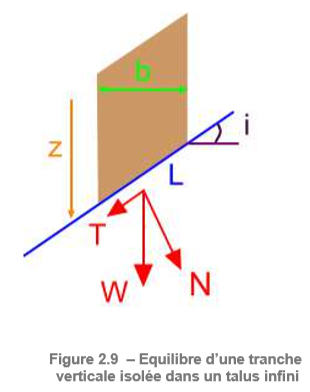
\includegraphics [scale=0.5]{pictures/ze.PNG}
\end{center}

On a déjà fait cette démonstration 100 fois, je vous la passe.

\underline{Remarque:} le massif peut être saturé sans qu'il y ait pour autant écoulement de son eau interstitielle (pente noyé ou fond marin).

La stabilité de la tranche dépendra de la capacité qu'aura le sol à résister aux efforts appliqués le long de la surface potentielle de glissement. Qui est caractérisé par $\tau_{max} = c' + (\sigma - u) tan \phi$.

Le coefficient de sécurité quantifie la marge vis-à-vis du glissement en exprimant le rapport entre la résistance et la sollicitation.

Pour un sol pulvérulent: $F_s = \frac{tan \phi'}{\tan i} > 1$ on constate qu'elle ne dépend plus du $\gamma$ donc identique pour toute inclinaison i de sol ayant le même angle de frottement $\phi'$.

Pour un sol avec cohésion, le coefficient diminue avec la profondeur jusqu'à atteindre 0 à l'infini pour un sol purement cohésif.

\subsubsection{Présence d'un écoulement souterrain}

L'eau est l'élément déterminant. Non seulement u n'est pas nul mais en plus u n'obéit plus à la loi hydrostatique. L'eau en mouvement ne peut plus s'apparenter à la poussée d'Archimède et doit se déterminer explicitement. La pression interstitielle se détermine sur base du réseau d'écoulement, en évaluant la différence de cote le long d'une équipotentielle (entre le point considéré et celui ou la pression est nulle).

Par trigonométrie: $u = mz \gamma_w cos^2i$ 

\begin{center}
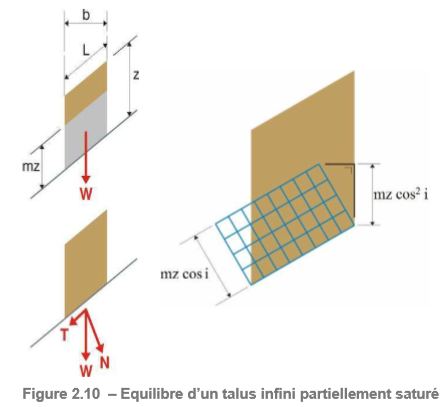
\includegraphics [scale=0.5]{pictures/zr.PNG}
\end{center}

$$ W = [(1-m) \gamma_n + m\gamma_{sat}]z b $$ 

On peut remettre tout ca dans l'équation du coefficient de sécurité.

Pour un cas pulvérulent: $F_s = \frac{\gamma'}{\gamma_{sat}} \frac{tan \phi'}{tan i}$

On observe que le coefficient d'écoulement se réduit d'environ de moitié par rapport à un talus sans écoulement (valeur du rapport des gamma).

\subsection{Rupture par rotation}

Ligne de glissement circulaire. Trois forces en présence: 
\begin{itemize}
    \item le poids W du massif
    \item la résultante des contraintes de cohésion C
    \item la résultante des contraintes de frottement R
\end{itemize}

\subsubsection{Contribution de la cohésion à la stabilité}

\begin{center}
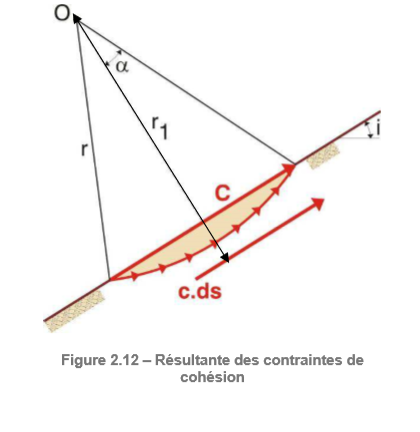
\includegraphics [scale=0.5]{pictures/34.PNG}
\end{center}

On suppose C non nul et $\phi = 0$. On recherche le vecteur équivalent aux termes de résistance dus à la cohésion c le long du cercle de glissement. Cette ligne d'action est à une distance r1 de O produisant un moment équivalent à la somme des moments dus aux termes individuels de résistance c au point O. On obtient donc :

$$ r_1 = \frac{cr2(r\alpha}{c2(r sin\alpha)} = \frac{a}{sin \alpha} r $$

Comme $\alpha > sin \alpha$ on sait que $r_1 > r$ et donc que la ligne d'action de C se trouve en dehors du cercle de rayon r.

\subsubsection{Contribution du frottement interne R à la stabilité}

On suppose $c=0$ nul et $\phi$ non nul. On recherche le vecteur R équivalent aux termes de résistance dus aux frottement interne le long du cercle de glissement.

\begin{center}
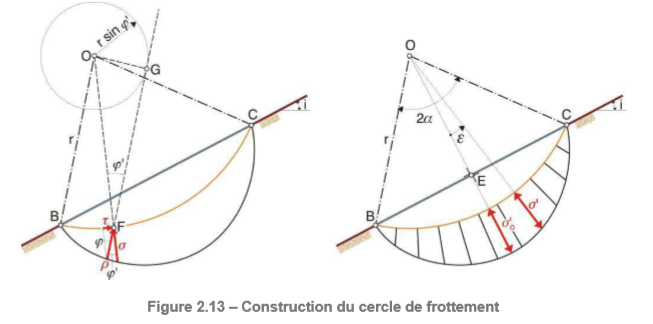
\includegraphics [scale=0.5]{pictures/Zt.PNG}
\end{center}

$|R| = \int \rho ds = \frac{1}{cos \phi} \int \sigma ds $

La grandeur R dépend de la répartition de $\sigma$ le long de la surface de glissement (qui est nulle en B et C mais maximale entre ces deux points, on choisira une loi de répartition entre ces deux points). Prenons une répartition symétrique par rapport à OE, la médiatrice de la corde BC.

La ligne d'action de R sera également tangente ) un cercle de centre O: le cercle de frottement modifié de rayon $\lambda (r sin \phi')$. Le paramètre $\lambda$ quantifie la modification du rayon du cercle de frottement. $\lambda$ se détermine en fonction de $\alpha$ par mise en évidence du moment en O.

$$\lambda = \sqrt{\frac{\alpha}{sin \alpha}}$$

\subsubsection{Sécurité de rotation d'un segment de cercle pour cohésion non nulle et $\phi$ = 0}

On suppose que le sol n'a aucune résistance au frottement et donc que la résistance est amenée par la cohésion. On vérifie si cela suffit à empêcher une rupture.

\begin{center}
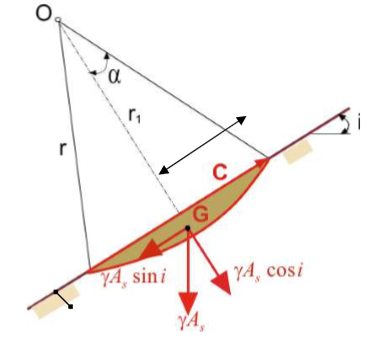
\includegraphics [scale=0.5]{pictures/ae.PNG}
\end{center}

On peut exprimer le coefficient de sécurité vis-à-vis de la rotation:

$$ FS_R = \frac{M_y}{M_z}=\frac{3 \alpha c}{\gamma sin^3\alpha sin i} $$ 

Pour D=cst et $FS_{min}$ pour $\alpha = 0\degree$ on obtient $FS_{R \alpha = 0} = \frac{c}{\gamma D} \frac{1.5}{sin i} = 1.5 FS_T$

On montre ainsi que dans un sol homogène cohésif, le facteur de sécurité de rotation est presque toujours plus élevé que le facteur de sécurité de translation (ne faisant pas intervenir la résistance du sol sur des profondeur associées aux émergences du mécanisme circulaire).

\subsubsection{Sécurité de rotation d'un segment de cercle pour c et $phi = 0$}

mouai (p15)

\section{Talus de hauteur limitée}

\subsection{Méthode globale du cercle de frottement}

Très semblable au cas de rupture par rotation dans un talus infini. La différence se note au niveau de la masse en mouvement, de son centre de gravité ainsi que de l'amplitude de l'angle de demi-ouverture $\alpha$.

\subsubsection{Contribution de la cohésion C à la stabilité}

\begin{center}
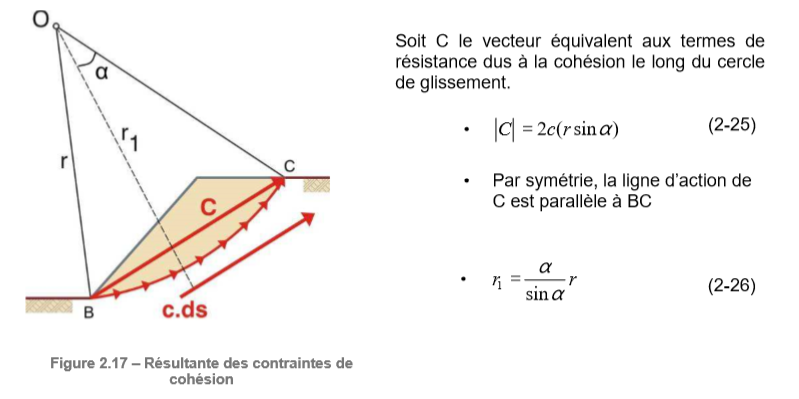
\includegraphics [scale=0.8]{pictures/t.PNG}
\end{center}

\subsubsection{Contribution du frottement interne R à la stabilité}

\begin{center}
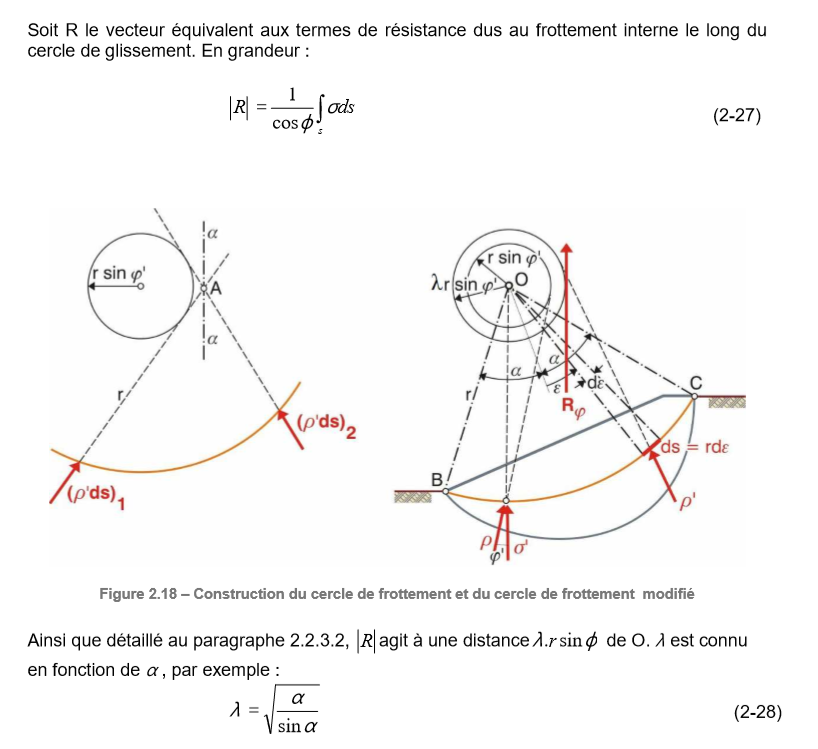
\includegraphics [scale=0.8]{pictures/t2.PNG}
\end{center}

\subsubsection{Recherche du coefficient de sécurité}

Dans la pratique, un massif ne devrait pas se trouver à la limite de l’équilibre car le calcul de stabilité consiste à rechercher, pour une surface potentielle de glissement, le coefficient de sécurité en espérant ne pas en trouver une valeur impliquant la rupture.

Méthode du cercle de frottement, on définit deux coefficients de sécurité:
\begin{itemize}
    \item $s_c$: portant sur la cohésion c
    \item $s_{\phi}$: portant sur l'angle de frottement $\phi$
\end{itemize}

\medskip

\begin{center}
\begin{tabular}{c|c}
$s_c = \frac{c'}{c'_b}$
                & $c_b$ cohésion nécessaire pour assurer la stabilité  \\
$s_{\phi} = \frac{tan \phi'}{tan \phi'_b}$
                & $phi_b$ angle de frottement nécessaire pour assurer la stabilité 
\end{tabular}
\end{center}

On dispose donc d'une infinité de couple de coefficients de sécurité pour une même surface de glissement considérée.

\begin{center}
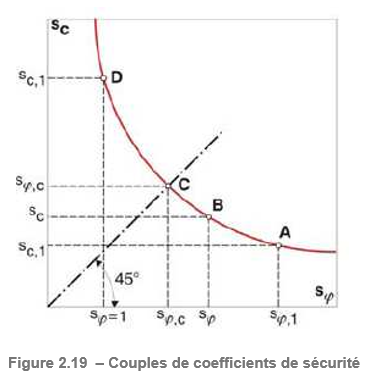
\includegraphics [scale=0.5]{pictures/csa.PNG}
\end{center}

\begin{itemize}
    \item cas A: on mobilise totalement la cohésion ($s_c = 1$).
    \item cas D: on mobilise totalement $\phi$ ($s_{\phi} = 1$).
    \item cas C: on égalise les coefficients.
\end{itemize}

\medskip

\underline{Cas A:} 
On en tire que $s_{\phi} = \frac{tan \phi'}{tan \phi'_b}$ et que $s_{c,1}=\frac{c'}{c'_b}$.

\subsection{Méthode de Fellenius (méthode des tranches)}

Consiste à diviser le talus en N tranches verticales, on considère les efforts concourant à l'équilibre et on exprime un équilibre limite de rotation global autour du centre du cercle de glissement (postulé).

hypothèse: sol homogène, surfaces de glissement potentielles circulaires.

On cherche les coefficients de sécurité des surfaces. On divise le massif sol en N tranches d'épaisseur unitaire.

\begin{center}
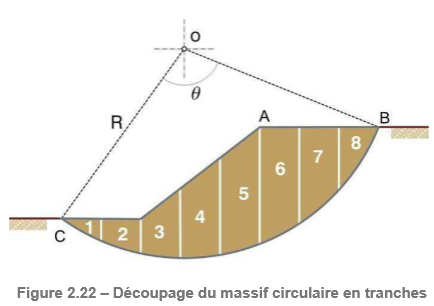
\includegraphics [scale=0.5]{pictures/222.PNG}
\end{center}

On y retrouve les forces suivantes : le poids propre ($W_n$), les réactions du milieu ($N_n$ et $S_n$) et les réactions sur les faces verticales ($X_n$, $E_n$, $X_{n+1}$ et $E_{n+1}$).

Le nombre d'inconnues étant supérieur au nombre d'équations, il est nécessaire de recourir à des hypothèses. La méthode de Fellenius néglige les forces inter-tranches normales ($E_n$) et tranchantes ($X_n$).

Le coefficient de sécurité au glissement exprime le rapport de la somme des moments opposant le glissement à la somme des moments le provoquant. 
\begin{itemize}
    \item Le moment agissant est du au poids : $\sum W_n Xn$
    \item Le moment résistant est dû aux forces de cohésion et de frottement. $\int_{arcBC} (c'+(\sigma-u)tan\phi)rds$
\end{itemize} 

\medskip

On obtient donc 

$$ F_s = \frac{R \sum[c'L_n+(W_n cos \alpha_n - u_n L_n) tan \phi}{\sum W_n x_n} $$

\subsection{Abaques de Taylor}

Pour un abaques rectiligne dans un massif homogène et en l'absence de pression d'eau, Taylor à établi des abaques donnant directement les coefficients et la position de la surfaces de glissement circulaire la plus défavorable. 

Il a distingué le cas de cercles de glissement passant par le pied du talus et de cercle de glissement "profond".

\subsubsection{Cercle de glissement de pied de talus}

Instabilité T par rapport à l'inclinaison i.Pour chaque valeur, l'abaque donne $\alpha_0$ et $\beta_0$ correspondant à la valeur maximale de l'indice de stabilité T.

\begin{center}
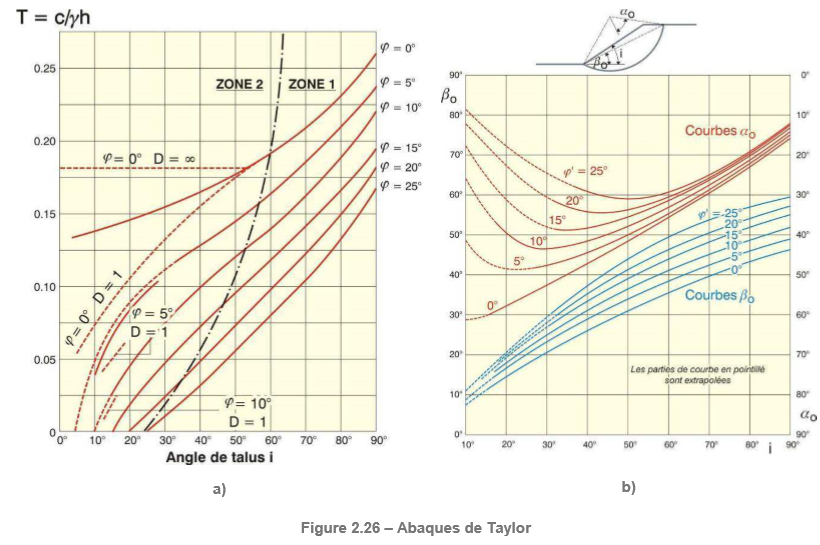
\includegraphics [scale=0.8]{pictures/at.PNG}
\end{center}

\begin{itemize}
    \item Zone I: $\alpha_0 < \beta_0$. Le centre O se trouve à gauche de la verticale de B. La surface de glissement ne passe jamais en dessous de l'horizontale du pied de talus. Dès lors que le sol situé sous cette horizontale soit plus résistant, la surface de glissement ne changera pas.
    \item Zone II: $\alpha_0 > \beta_0$. Si le sol sous l'horizontal est plus résistant, la surface la plus défavorable sera refoulée vers le haut et recoupera le talus. Condition géométrique supplémentaire, on aura donc une cohésion et un donc un indice de sécurité plus faible.
\end{itemize}

\subsubsection{Cercle de glissement profond}

Il peut être caractérisé par 3 paramètres. La longueur L, la profondeur D et le rayon r (ou d'autres).

\begin{center}
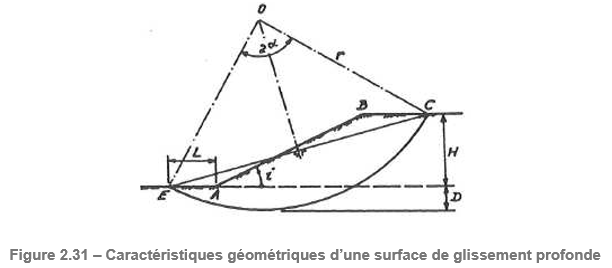
\includegraphics [scale=0.8]{pictures/231.PNG}
\end{center}

\underline{cas 1: $\phi = 0$} 
la surface la plus défavorable est un cercle de rayon infini. Indice de stabilité constant et représenté par la droite horizontale pointillé de l'abaque précédent. On peut en déduire que la surface de glissement profonde est la plus défavorable lorsque $i<53\degree$ tandis que la surface de glissement de pied de talus est la plus défavorable lorsque $i>53\degree$ (C'est très théorique, on rencontre toujours une couche résistante avant l'infini).

L'abaque suivant défini le mécanisme de rupture sur base de contraintes géométriques (latérale et profondeur).

\begin{center}
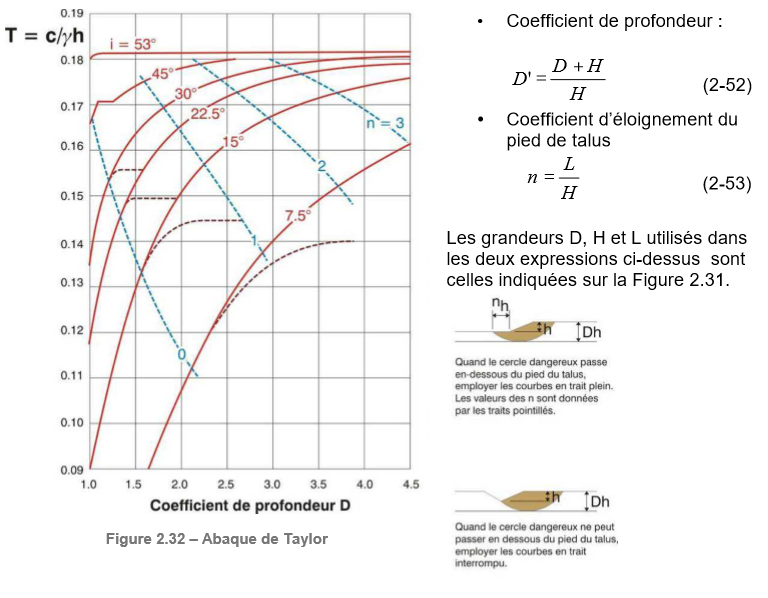
\includegraphics [scale=0.8]{pictures/232.PNG}
\end{center}

Les traits pleins donne les valeurs de l'indice de stabilité de surface profondes. Il arrive que par exemple suite à la surcharge du sol en pied de talus, la surface de glissement profonde ne puisse se développer (ces courbes sont tracés en pointillés).

\underline{cas 2: $\phi \neq 0$} 
Les surfaces de glissement profondes ne seront plus défavorables que les surfaces de glissement en pied de talus que pour des valeurs $\phi' \leq 5\degree$ (trait interrompu du premier abaque).

\section{Considérations essentielles pour la conception}

\subsection{Sécurité et choix des paramètres de cisaillement}

Il dépend des enjeux, de la connaissance géologique, de la confiance du concepteur,... Il varie de 1,2 à 1,5. 

\underline{Sol drainé ?}
\begin{itemize}
    \item état saturé ou non du sol
    \item la nature du sol saturé (coefficient de consolidation)
    \item taille du mécanisme de rupture (longueur des chemins de drainage)
    \item le passé géologique (degré de surconsolidation ou glissement passé)
    \item la manière de fabrication (déblai entraîne une diminution des contraintes totales, remblai c'est l'inverse).
    \item la vitesse de construction
    \item les charges opérationnelles (ex: barrage = construction, vidange, remplissage, retenue)
    \item la durée du talus dans le temps
\end{itemize}

essai triaxial non nécessaire pour un mode opératoire drainé (CD), essentiellement non drainé (UU) ou non drainé après consolidation (CU). Certains problèmes peuvent requérir deux jeux de paramètres venant d'une analyse à court terme (non drainée) et à long terme (drainée).

Rappelons par exemple comment déterminer les paramètres de rupture avec un essai de cisaillement simple (toujours préféré l'essai triaxial, mieux pour dimensionner u). On connaît $\sigma'$ le long de la surface de cisaillement. On peut donc faire un graphe $\tau - \sigma$ avec les points correspondant aux résistances de cisaillement $s_f$ et $s_r$ (pic résiduelle). On fait ca pour diverse valeur de $\sigma'$ et on trouve les efforts intrinsèques correspondant aux valeurs de pics résiduelles. On en déduit les caractéristiques de cisaillement.

Le pic résiduel est utilisé si le massif à déjà connu un glissement par le passé.

\begin{center}
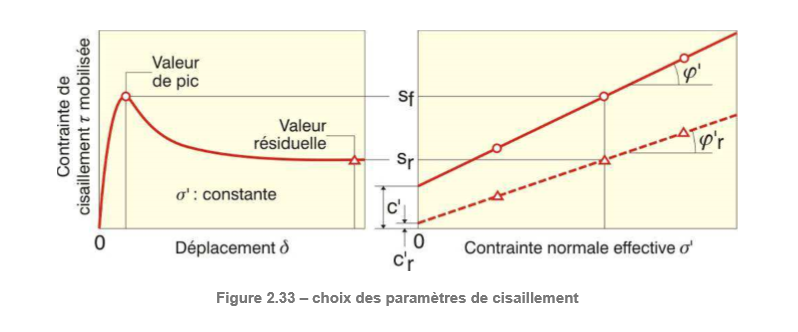
\includegraphics [scale=0.8]{pictures/233.PNG}
\end{center}

\subsection{Rôle de l'eau}

Il faudra se préoccuper de savoir si l'eau est en mouvement ou non. Différentes situations possibles:

\begin{center}
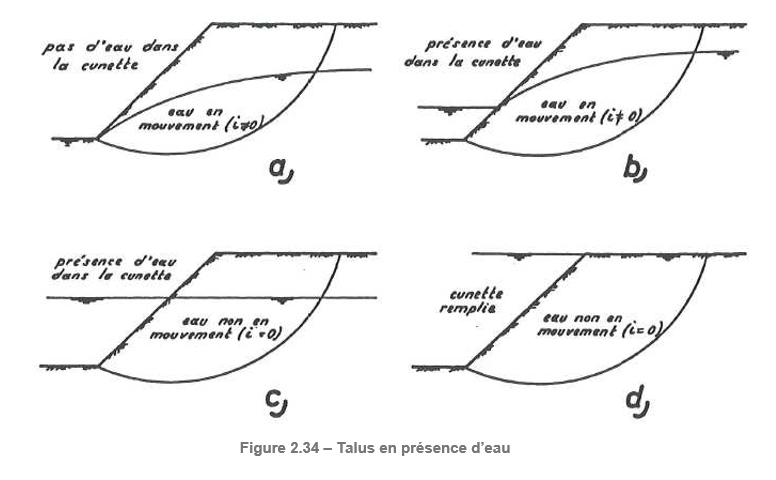
\includegraphics [scale=0.8]{pictures/234.PNG}
\end{center}

\subsubsection{Eau au repos}

ex: talus immergé (barrage à terre,...).
Les résultantes de pression ne provoquent pas de contraintes tangentielles. Il suffit de vérifier l'équilibre du massif déjaugé ($\gamma'$ au lieu de $\gamma_{sat}$).

\begin{center}
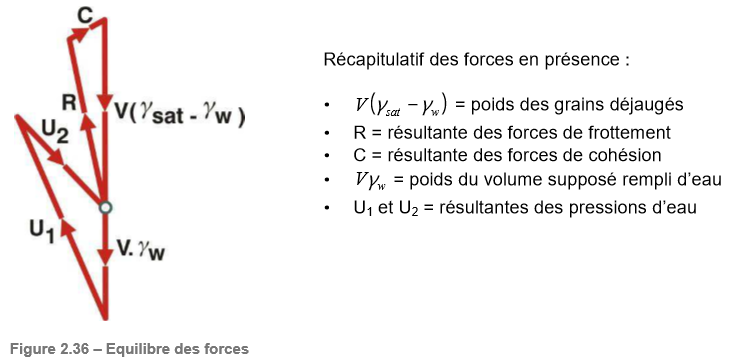
\includegraphics [scale=0.8]{pictures/236.PNG}
\end{center}

\subsubsection{Vidange rapide}

Les contraintes inter granulaires varient peu à court terme. La résultante des forces de frottement R reste inchangée. Mais comme la résultante des pressions d'eau extérieures s'annule, elle ne peut contribuer à la stabilité d'ensemble. D'autre part la charge de l'eau n'étant plus la, la pression interstitielle U1 diminue à Ua. Il reste donc le poids du talus et Ua qui doivent être en équilibre grâce à un supplément de cohésion Ca.

\begin{center}
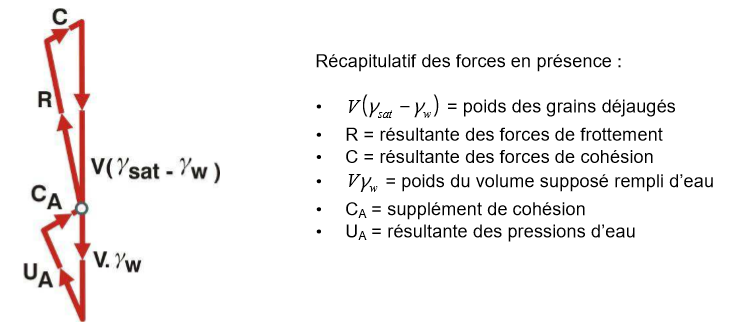
\includegraphics [scale=0.8]{pictures/21.PNG}
\end{center}

En résumé, dans le cas de la vidange rapide on prendra pour angle de frottement, la valeur fictive ainsi définie pour calculer le coefficient de sécurité.

\subsubsection{Écoulement permanent}

On détermine le régime d'écoulement au sein du talus en résolvant l'équation de Laplace sur le potentiel. Cela permet de connaître la pression interstitielle au sein du massif.

On considère deux forces:
\begin{itemize}
    \item La force W du à l'eau dans la cuvette
    \item La force Nw réultante des contraintes dans la phase liquide le long de l'arc.
\end{itemize}

On effectue ensuite les étapes suivantes:
\begin{itemize}
    \item On cherche la résultante P du poids G du massif, de la force W et de Nw.
    \item On détermine $T_c$ et $R_{\phi}$
\end{itemize}

Il suffit finalement de remplacer G par la force P et de continuer le calcul sans plus se préoccuper des pressions d'eau.

\subsection{Abaques de Kérisel}

Abaques permettant de calculer le coefficient de sécurité minimum $s_{\phi,c}$ correspondant à la surface de glissement la plus défavorable.

Hypothèses: 
\begin{itemize}
    \item lignes de courant rectilignes, parallèle entre elles et d'une inclinaison $\lambda$ avec l'horizontale
    \item ligne de courant passe par le pied du talus
    \item Poids spécifique des grains $\gamma_s = 27kN/m^3$
    \item Poids spécifique de l'eau $\gamma_w = 10kN/m^3$
    \item Pourcentage des vides $n=33\%$
    \item le sol est saturé car c'est plus défavorable qu'un sol sec.
\end{itemize}

On trouve ainsi le poids volumétrique sec $\gamma_d = 18kN/m^3$ et le poids volumétrique saturé $\gamma_{sat} = 21.3 kN/m^3$

\begin{center}
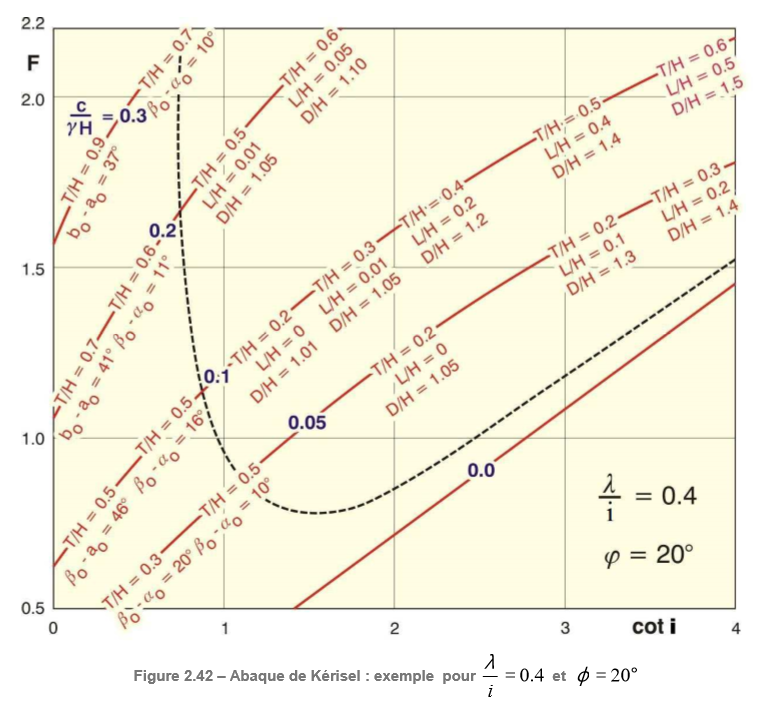
\includegraphics [scale=0.8]{pictures/242.PNG}
\end{center}

On observe que:
\begin{itemize}
    \item Le coefficient de sécurité minimal se trouve en ordonnées avec cot(i) en abscisses.
    \item Chaque abaque est caractérisé par une valeur de $\phi'$ et un rapport de $\frac{\lambda}{i}$ dont on traite 6 valeurs.
    \item Les courbes sont définie par un paramètre $I_s = \frac{c'}{\gamma_{sat} H}$
    \item La zone 1 correspond à une surface de glissement passant sous l'horizontale et la zone 2, un glissement entièrement au dessus de l'horizontale (délimité en pointillé (i=0)).
    \item On peut connaître la position de la surface la plus défavorable le long des lignes $I_s$ = constante:
    \begin{itemize}
        \item Zone 1: $n_D = \frac{D}{H}$, $n_L = \frac{L}{H}$ et $n_S = \frac{S}{H}$
        \item Zone 2: $n_s$ et $\beta$
    \end{itemize}
\end{itemize}

\subsection{Abaques de Cousin}

Méthode plus complète que celle de Taylor permet une détermination plus directe du coefficient de sécurité grâce à l'introduction des paramètres adimensionnels suivants: le nombre de stabilité (Nf) et le paramètre $\lambda_{c\phi}$ qui exprime le rapport des résistances au cisaillement imputable au frottement interne et imputable à la cohésion.

Le coefficient $r_u$ est appelé le coefficient de pression interstitielle et permet de décrire la distribution de la pression interstitielle dans un talus avec u,$\gamma$ et H.

\begin{center}
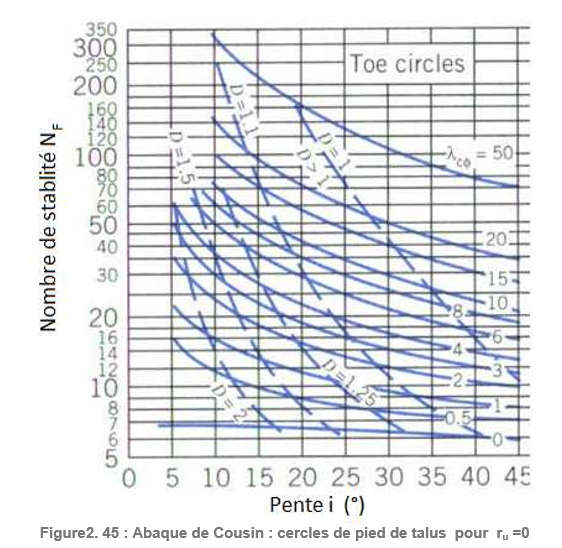
\includegraphics [scale=0.8]{pictures/245.PNG}
\end{center}

On remarque une diminution de la sécurité d'un talus lorsque rien n'empêche le cercle de glissement de s'approfondir (facteur de profondeur supérieur à 1 (D>1)).
